\section{System instructions}
\label{app:system_instructions}
In order to run the core system the following dependencies are required:
\begin{itemize}
\item Python 2.7
\item Theano
\item Numpy
\item Unirest
\end{itemize}

The system has only been tested with Ubuntu 14.04, but it should be possible to run on both Windows and Linux as long as the listed dependencies have been installed. Ubuntu is highly recommended because of a more convenient installation process. \\

A Nvidia GPU is also highly recommended for running the system. In most instances a GPU can give considerable speed improvements when training compared to a CPU. This is critical when having to deal with large datasets and models with millions of parameters. In order for Theano to efficiently use your GPU while training, CUDA Toolkit has to be installed. \\

A graphical user interface can also be utilized for monitoring training. Running experiments can be stopped from this user interface, as well as a debugging option which display examples and model predictions. In addition all experiment data is stored as JSON, and can be viewed in the user interface. This includes, a loss graph, precision and recall curve and hyperparameters used while training. \\

The monitoring system can either be run locally, or installed on a server. All communication between the core system and the monitoring system is done by HTTP messaging. To enable monitoring, enable\_gui should be set to true in the core system's config file.

Utilizing this monitoring system requires these dependencies:
\begin{itemize}
\item Node.js
\item MongoDB
\end{itemize}

For installation instructions, see Appendix \ref{app:monitorInstall} and Appendix \ref{app:ubuntuInstall}. Alternatively, installation guides have been included in the README files of the repositories. The URL of these repositories are listed below:

\begin{itemize}
\item https://github.com/olavvatne/CNN
\item https://github.com/olavvatne/ml-monitor
\end{itemize} 


\section{System Installation Guide - Ubuntu}
\label{app:ubuntuInstall}
This guide will help you install all dependencies required for running Theano with a GPU, which should be done in order to run the system. \\
\noindent Install all dependencies:
\begin{lstlisting}[language=bash]
  $ sudo apt-get install -y gcc g++ gfortran build-essential git
   wget linux-image-generic libopenblas-dev python-dev python-pip 
   python-nose python-numpy python-scipy  
\end{lstlisting}
~\\

\noindent Install Theano:
\begin{lstlisting}[language=bash]
  $ sudo pip install --upgrade --no-deps 
  git+git://github.com/Theano/Theano.git
\end{lstlisting}
~\\

\noindent Download Cuda 7 toolkit:
\begin{lstlisting}[language=bash]
  $ sudo wget http://developer.download.nvidia.com/
  compute/cuda/repos/ubuntu1404/x86_64/
  cuda-repo-ubuntu1404_7.0-28_amd64.deb
\end{lstlisting}
~\\

\noindent Depackage Cuda:
\begin{lstlisting}[language=bash]
  $ sudo dpkg -i cuda-repo-ubuntu1404_7.0-28_amd64.deb  
\end{lstlisting}
~\\

\noindent Install the cuda driver:
\begin{lstlisting}[language=bash]
  $ sudo apt-get update
  $ sudo apt-get install -y cuda  
\end{lstlisting}
~\\

\noindent Append path for Cuda nvcc in PATH and add LD\_LIBRARY\_PATH in the .bashrc file (see Table \ref{tab:install_bash_paths}). Then do a reboot:

\FloatBarrier
\begin{table}[!htbp]
\caption[Paths to include]{Paths to include.}
\begin{center}
\begin{adjustbox}{max width=\textwidth}
\begin{tabular}{ l }
  \hline			
  export PATH=(...):/usr/local/cuda/bin  \\
  export LD\_LIBRARY\_PATH=/usr/local/cuda/lib64 \\
  \hline  
\end{tabular}
\end{adjustbox}
\end{center}
\label{tab:install_bash_paths}
\end{table}
\FloatBarrier

\noindent  Create a theano config file as illustrated in Table \ref{tab:install_theano_config_file}. Name this file .theanorc and place it in your home directory:\\

\FloatBarrier
\begin{table}[!htbp]
\caption[Theano config file]{Theano config file.}
\begin{center}
\begin{adjustbox}{max width=\textwidth}
\begin{tabular}{ l }
  \hline			
  ~[global] \\
  floatX=float32 \\
  device=gpu \\
  mode=FAST\_RUN \\
  \\
  ~[nvcc] \\
  fastmath=True \\
  \\
  ~[cuda] \\
  root=/usr/local/cuda \\
  \hline  
\end{tabular}
\end{adjustbox}
\end{center}
\label{tab:install_theano_config_file}
\end{table}
\FloatBarrier

\noindent Clone CNN repository, which contains the core system:
\begin{lstlisting}[language=bash]
  $ git clone https://github.com/olavvatne/CNN.git 
\end{lstlisting}
~\\

\noindent Navigate to the root of the cloned repository. Create a secret.py file, and put the token created for the Monitoring Interface in a variable. See Appendix \ref{app:monitorInstall}:
\begin{lstlisting}[language=bash]
  token = "Bearer " + ml-monitor-token
\end{lstlisting}
~\\

\section{Monitoring Interface Installation Guide - Ubuntu}
\label{app:monitorInstall}
This guide outlines the steps required for setting up the monitoring interface. This guide can also be found in the repository's README file. Some of the steps are slightly different for Windows. \\

\noindent Clone the ml-monitor repository:
\begin{lstlisting}[language=bash]
  $ git clone https://github.com/olavvatne/ml-monitor.git
\end{lstlisting}
~\\

\noindent Install Node.js on your system:
\begin{lstlisting}[language=Python]
  $ sudo apt-get update
  $ sudo apt-get install nodejs
\end{lstlisting}
~\\

\noindent Install npm package manager:
\begin{lstlisting}[language=bash]
    Install npm package manager:
\end{lstlisting}
~\\

\noindent Install MongoDB:
\noindent Navigate to ml-monitor, and install the dependencies of ml-monitor:
\begin{lstlisting}[language=bash]
    $ npm install
\end{lstlisting}
~\\

\noindent Before running ml-monitor, some database collections and a user have to be created in Mongo Shell:
\begin{lstlisting}[language=bash]
    $ export LC_ALL=C (Optional. Might be necessary)
    $ mongo
\end{lstlisting}
~\\

\noindent Inside Mongo Shell, first create a new database:
\begin{lstlisting}[language=bash]
    > use ml-monitor
\end{lstlisting}
~\\

\noindent Then create the database collections required by ml-monitor:
\begin{lstlisting}[language=bash]
    > db.createCollection('experimentlist')
    > db.createCollection('userlist')
    > db.createCollection('grouplist')
\end{lstlisting}
~\\

\noindent Create a user. The authentication system is very simple, so remember to create a long random string of characters as token:
\begin{lstlisting}[language=bash]> 
    db.userlist.insert(
    {"user": "ola", "password": "password", "token": "String"})
\end{lstlisting}
~\\

\noindent Finally, insert the default group, that new experiments will be assigned to:
\begin{lstlisting}[language=bash]
    > db.grouplist.insert(
    {"name": "unassigned", "gid": "0", "date_created": new Date()})
\end{lstlisting}
~\\

\noindent To start the system, run:
\begin{lstlisting}[language=bash]
    $ npm run start
\end{lstlisting}

\section{Experiment tools overview}
\label{app:tools}
All tools which have been created for this thesis are listed below. The source code can be found inside the tools module of the road detection system's repository.
\begin{itemize}
\item measurement.precisionrecall.py\\
The tool creates the precision and recall curve. Command line options can be supplied.
\item layer.visualize.py\\
Opens a params.pkl file, containing the weight and hyperparameter configuration of a trained network, and created a visualization of the kernels from the network's input layer.
\item distribution.curriculum\_diff.py\\
Samples patches and create a histogram showing a patch dataset difficulty estimate distribution. Useful for setting threshold $D_\theta$. Also useful for verifying the content in a curriculum patch dataset stage.
\item distribution.dataset\_std.py\\
Tool for finding an estimate of dataset's standard deviation. Used by contrast normalization in the pre-processing step.
\item distribution.label\_dist\\
Counts the percentage of road label pixels in a dataset.
\item curriculum.dataset\_create.py\\
Tool for pre-generate a curriculum patch dataset. Command line options can be passed, to select a teacher, the thresholds $D_\theta$, the teachers optimal thresholding value, and dataset. The tool also comes with a baseline option which generate a staged patch dataset without curating the content of each stage.
\item convert.alpha.py\\
Converts a RGB dataset to RGBA. Python module PIL quirk, which makes RGBA better when rotating the aerial images. Areas not covered by pixels after a rotation, set to transparent with RGBA. With RGB, these pixels are set to black, which results in a lot of patch examples with no content.
\item figure.average\_compare.py\\
Averages experiment runs, and plots the averaged MSE loss and precision and recall curve from the test dataset. The tool also marks the precision and recall breakeven point in the Figure. The resulting figures are used for comparison purposes in this thesis.
\item figure.average\_loss.py\\
Averages the test, validation and training loss from experiment replicates, and plots the result in a figure. 
\item figure.average\_noise\_levels\\
Average the final MSE loss for each replicate experiment, and precision and recall breakeven. 
The figures created by this tools, show the MSE loss and breakeven, over increasing levels of label noise.
\end{itemize}

\section{Road Detection Systems Results}
\label{app:roaddetectionresults}
In this appendix results from the best performing convolutional neural networks are displayed. The precision and recall breakeven point of the model trained on the Massachusetts Roads Dataset is 0.863. Whereas, the breakeven point for the best model trained on the Norwegian Roads Dataset is 0.765.  \\

\begin{figure}[H]
\begin{subfigure}{0.23\textwidth}
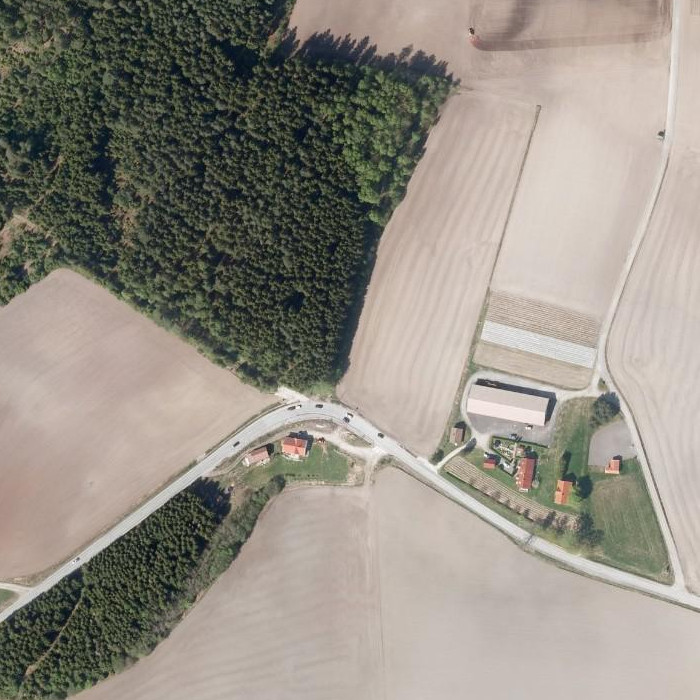
\includegraphics[width=\textwidth]{figs/appendix/img1151.jpg}
\caption{ Image. }
\vspace{0.2cm} % separation vertically between the subfigures
\end{subfigure}
\hspace*{\fill} % separation between the subfigures
\begin{subfigure}{0.23\textwidth}
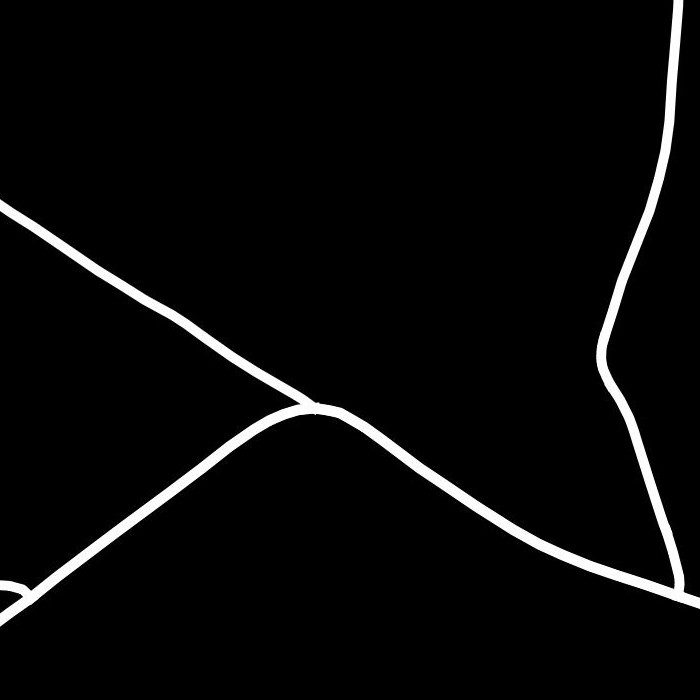
\includegraphics[width=\textwidth]{figs/appendix/label1151.jpg}
\caption{ Label. }
\vspace{0.2cm} % separation vertically between the subfigures
\end{subfigure}
\hspace*{\fill} % separation between the subfigures
\begin{subfigure}{0.23\textwidth}
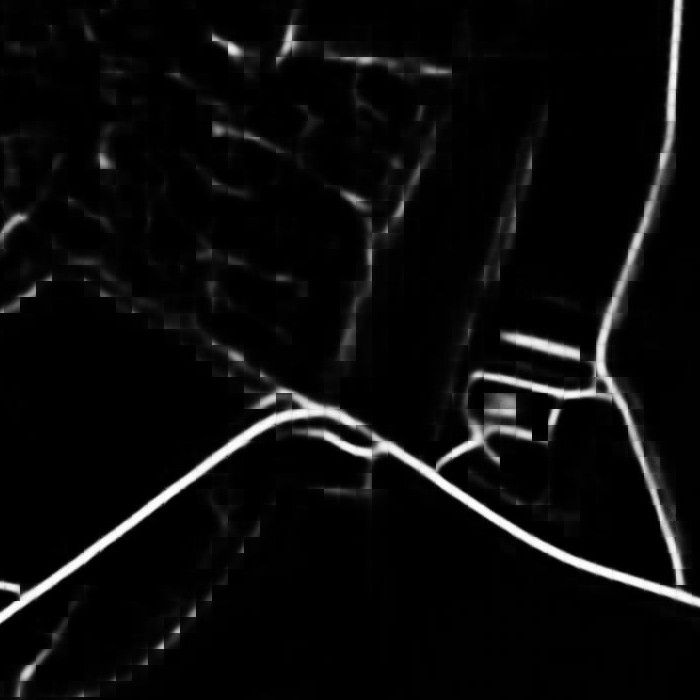
\includegraphics[width=\textwidth]{figs/appendix/pred1151.jpg}
\caption{ Prediction. }
\vspace{0.2cm} % separation vertically between the subfigures
\end{subfigure}
\hspace*{\fill} % separation between the subfigures
\begin{subfigure}{0.23\textwidth}
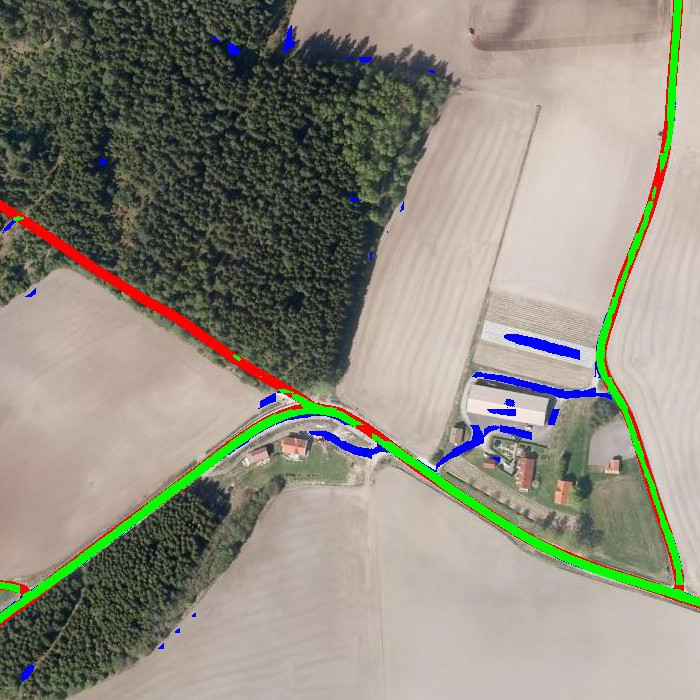
\includegraphics[width=\textwidth]{figs/appendix/hit1151.jpg}
\caption{ Hits. }
\vspace{0.2cm} % separation vertically between the subfigures
\end{subfigure}
\begin{subfigure}{0.23\textwidth}
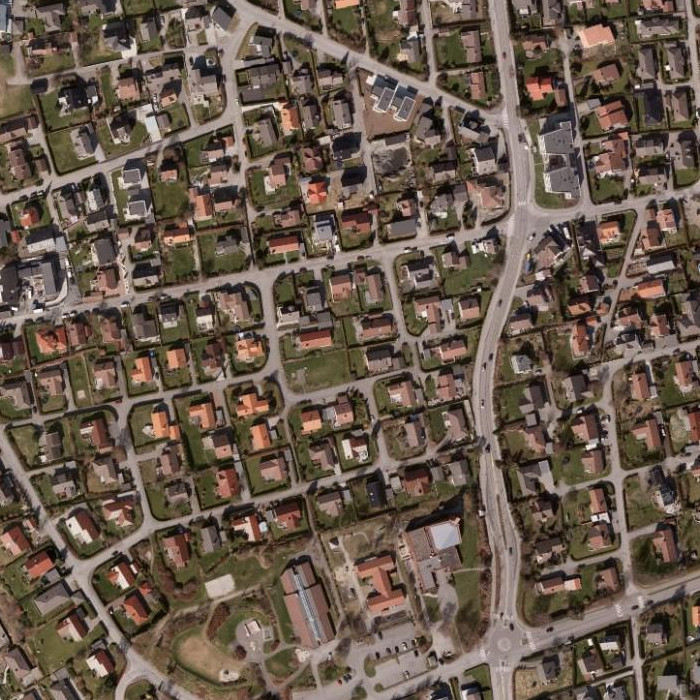
\includegraphics[width=\textwidth]{figs/appendix/img1160.jpg}
\caption{ Image.}
\vspace{0.2cm} % separation vertically between the subfigures
\end{subfigure}
\hspace*{\fill} % separation between the subfigures
\begin{subfigure}{0.23\textwidth}
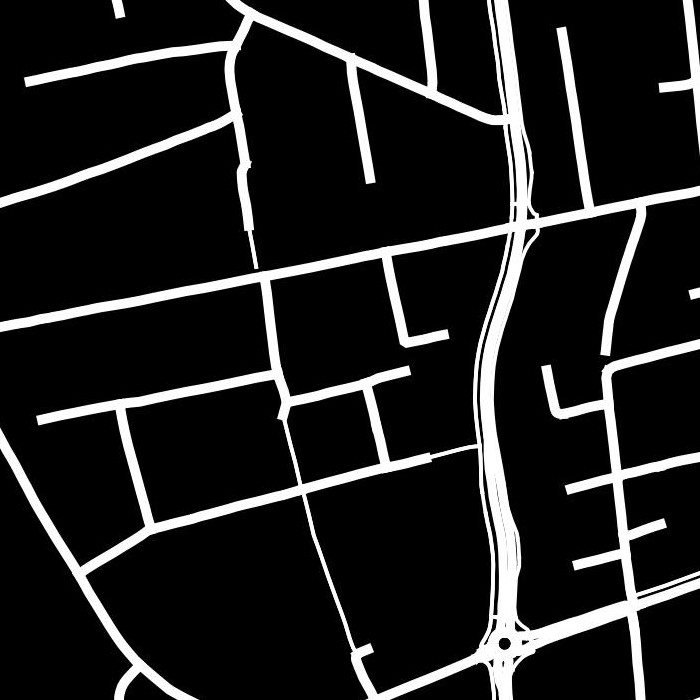
\includegraphics[width=\textwidth]{figs/appendix/label1160.jpg}
\caption{Label}
\vspace{0.2cm} % separation vertically between the subfigures
\end{subfigure}
\hspace*{\fill} % separation between the subfigures
\begin{subfigure}{0.23\textwidth}
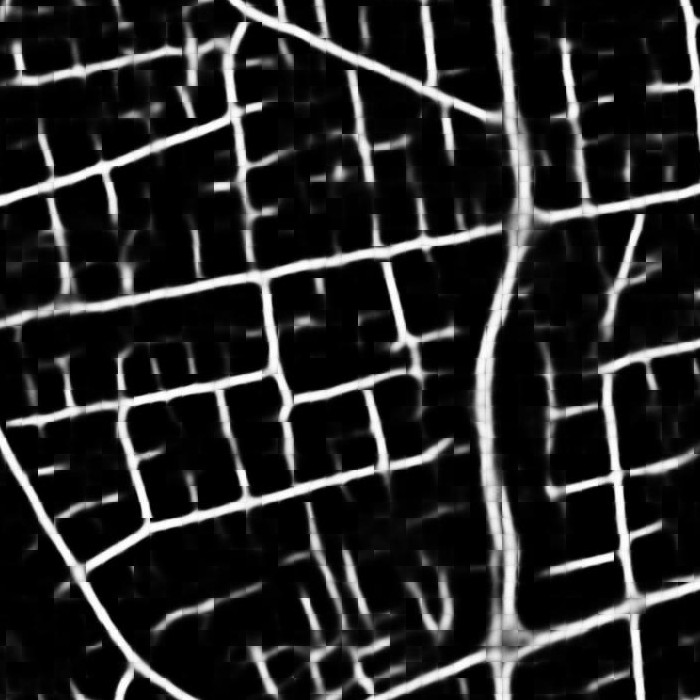
\includegraphics[width=\textwidth]{figs/appendix/pred1160.jpg}
\caption{Prediction.}
\vspace{0.2cm} % separation vertically between the subfigures
\end{subfigure}
\hspace*{\fill} % separation between the subfigures
\begin{subfigure}{0.23\textwidth}
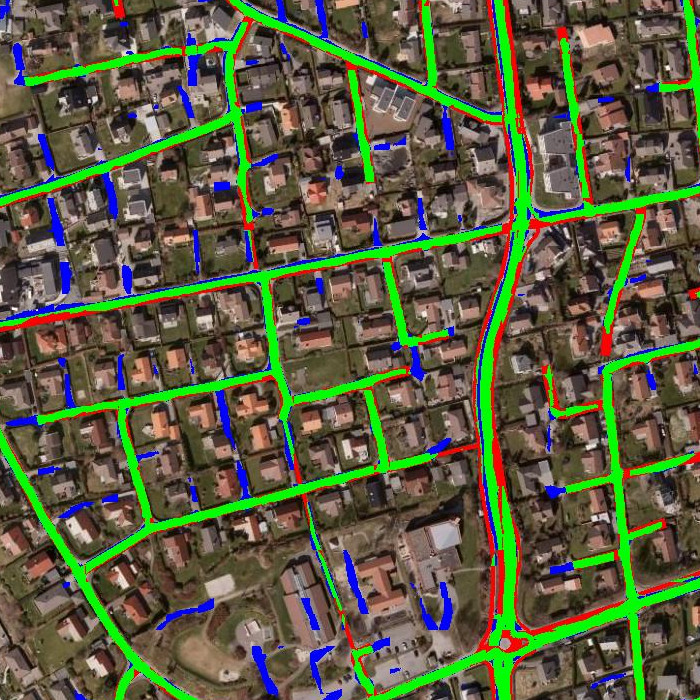
\includegraphics[width=\textwidth]{figs/appendix/hit1160.jpg}
\caption{Hits.}
\vspace{0.2cm} % separation vertically between the subfigures
\end{subfigure}
\caption[Norway Road extraction results 1]{Road extraction results 1 from the Norwegian Roads Dataset} \label{fig:Norway_app_results1}
\end{figure}

\begin{figure}[H]
\begin{subfigure}{0.23\textwidth}
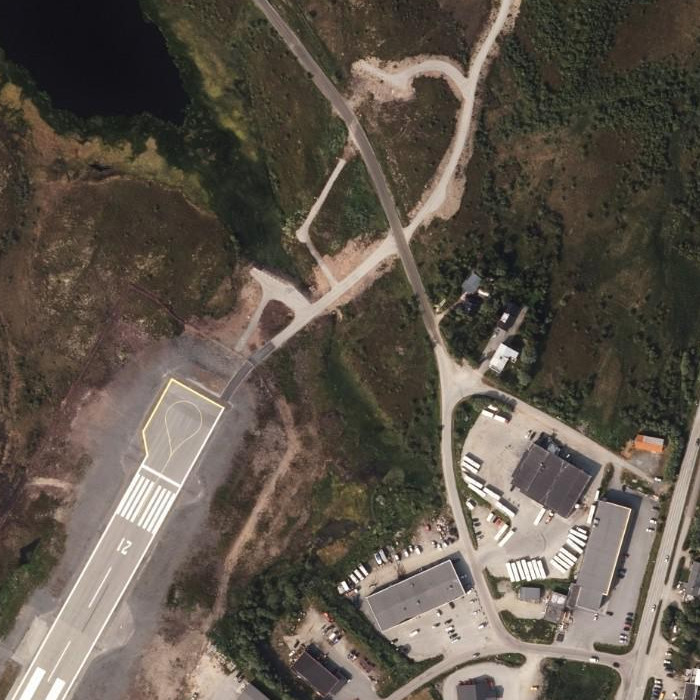
\includegraphics[width=\textwidth]{figs/appendix/img1205.jpg}
\caption{ Image. }
\vspace{0.2cm} % separation vertically between the subfigures
\end{subfigure}
\hspace*{\fill} % separation between the subfigures
\begin{subfigure}{0.23\textwidth}

\includegraphics[width=\textwidth]{figs/appendix/label1205.jpg}
\caption{ Label. }
\vspace{0.2cm} % separation vertically between the subfigures
\end{subfigure}
\hspace*{\fill} % separation between the subfigures
\begin{subfigure}{0.23\textwidth}
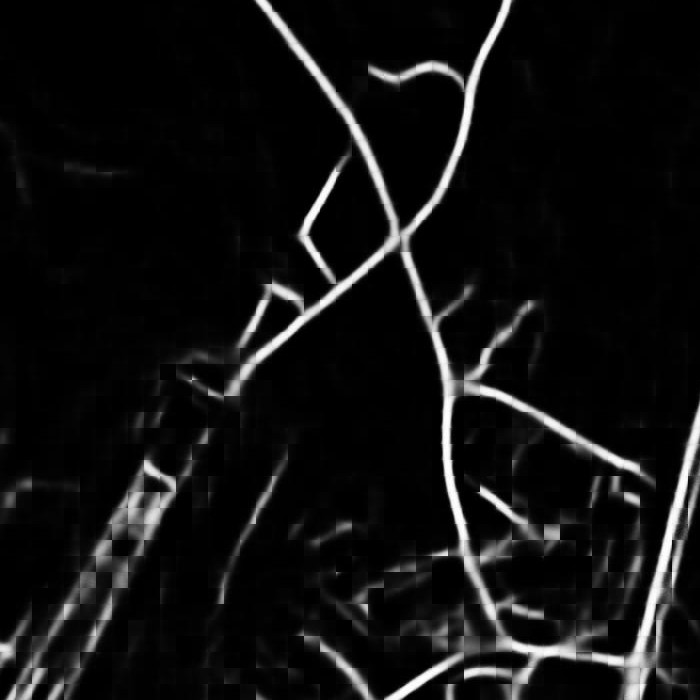
\includegraphics[width=\textwidth]{figs/appendix/pred1205.jpg}
\caption{ Prediction. }
\vspace{0.2cm} % separation vertically between the subfigures
\end{subfigure}
\hspace*{\fill} % separation between the subfigures
\begin{subfigure}{0.23\textwidth}
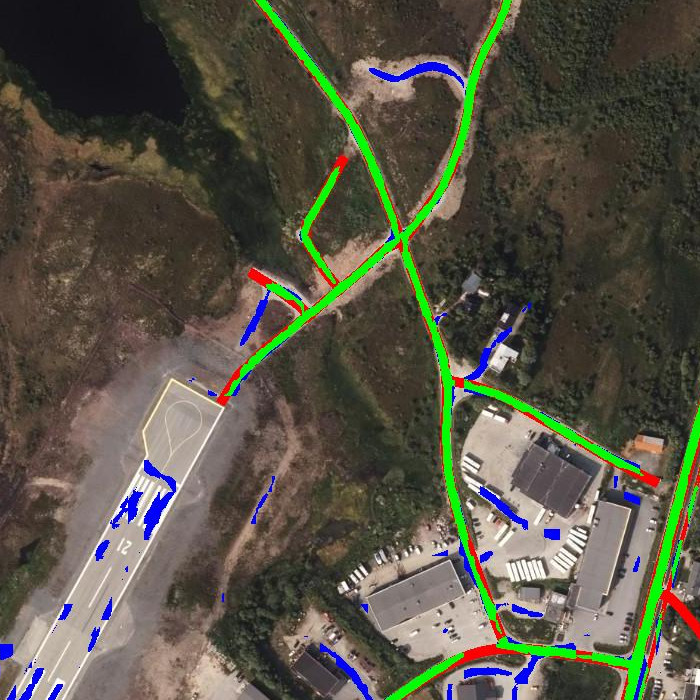
\includegraphics[width=\textwidth]{figs/appendix/hit1205.jpg}
\caption{ Hits. }
\vspace{0.2cm} % separation vertically between the subfigures
\end{subfigure}
\begin{subfigure}{0.23\textwidth}
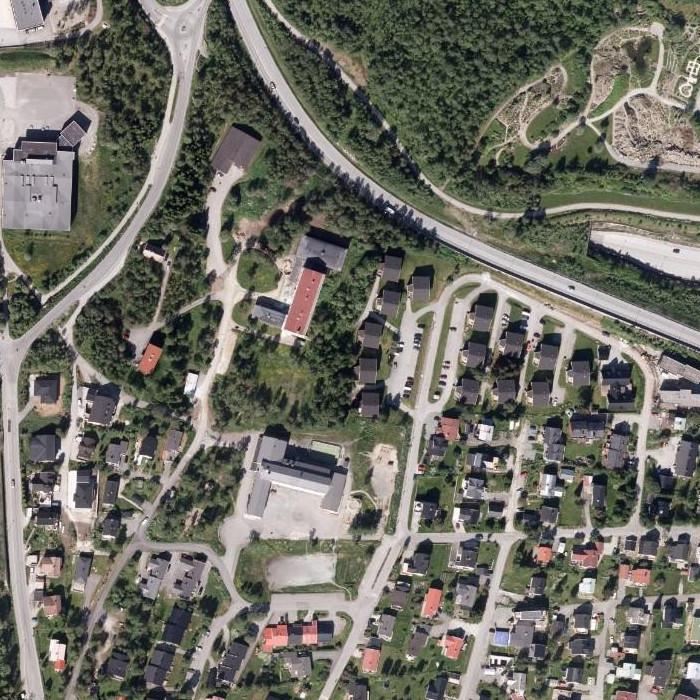
\includegraphics[width=\textwidth]{figs/appendix/img1217.jpg}
\caption{ Image.}
\vspace{0.2cm} % separation vertically between the subfigures
\end{subfigure}
\hspace*{\fill} % separation between the subfigures
\begin{subfigure}{0.23\textwidth}

\includegraphics[width=\textwidth]{figs/appendix/label1217.jpg}
\caption{Label}
\vspace{0.2cm} % separation vertically between the subfigures
\end{subfigure}
\hspace*{\fill} % separation between the subfigures
\begin{subfigure}{0.23\textwidth}
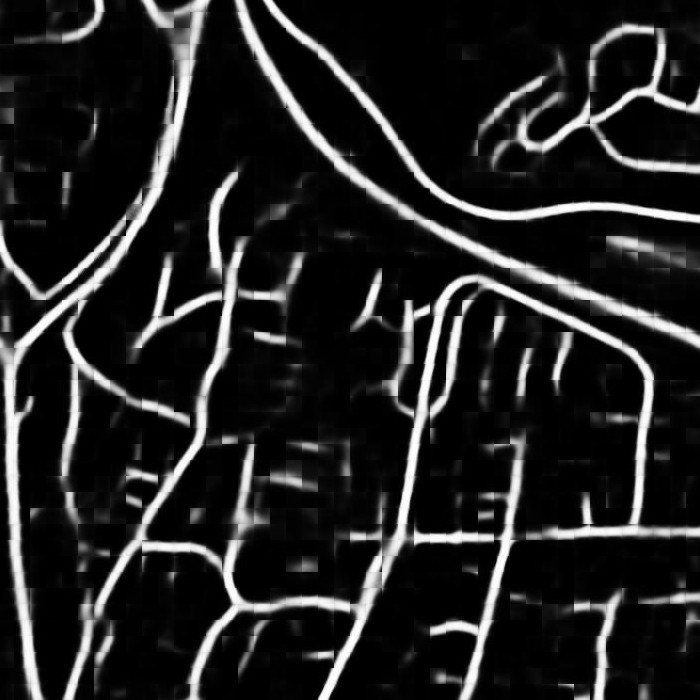
\includegraphics[width=\textwidth]{figs/appendix/pred1217.jpg}
\caption{Prediction.}
\vspace{0.2cm} % separation vertically between the subfigures
\end{subfigure}
\hspace*{\fill} % separation between the subfigures
\begin{subfigure}{0.23\textwidth}
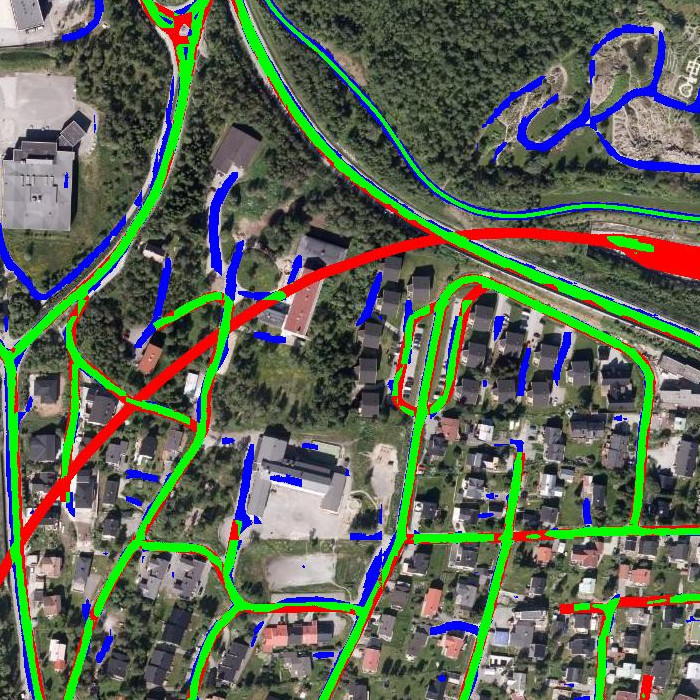
\includegraphics[width=\textwidth]{figs/appendix/hit1217.jpg}
\caption{Hits.}
\vspace{0.2cm} % separation vertically between the subfigures
\end{subfigure}
\caption[Norway Road extraction results 2]{Road extraction results 2 from the Norwegian Roads Dataset.} \label{fig:Norway_app_results2}
\end{figure}

\begin{figure}[H]
\begin{subfigure}{0.23\textwidth}
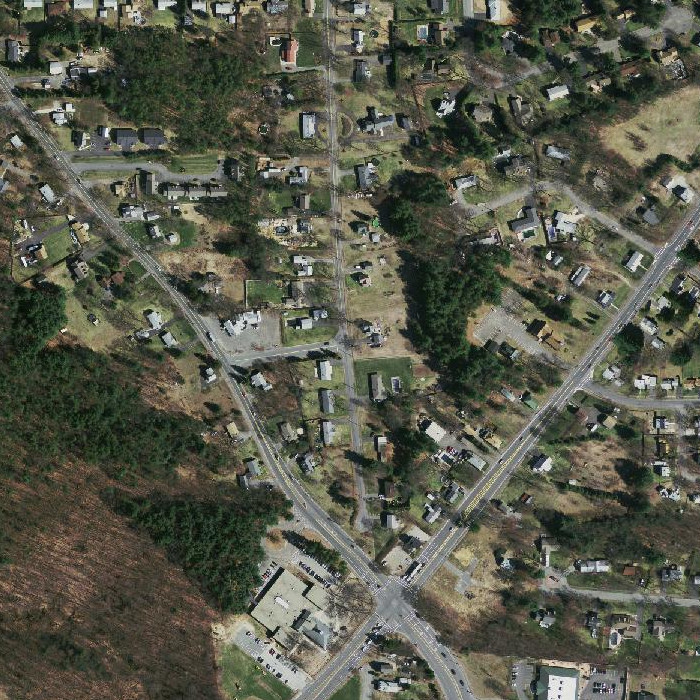
\includegraphics[width=\textwidth]{figs/appendix/img11128870_15.jpg}
\caption{ Image. }
\vspace{0.2cm} % separation vertically between the subfigures
\end{subfigure}
\hspace*{\fill} % separation between the subfigures
\begin{subfigure}{0.23\textwidth}
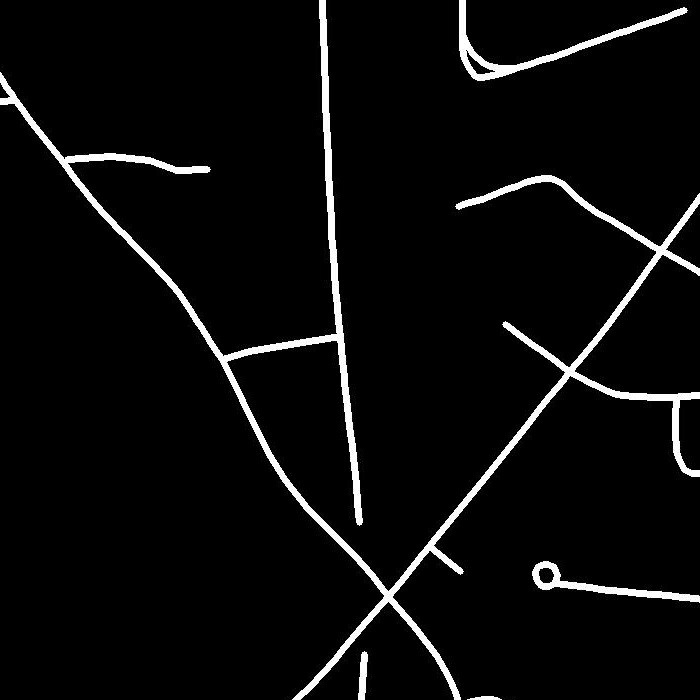
\includegraphics[width=\textwidth]{figs/appendix/label11128870_15.jpg}
\caption{ Label. }
\vspace{0.2cm} % separation vertically between the subfigures
\end{subfigure}
\hspace*{\fill} % separation between the subfigures
\begin{subfigure}{0.23\textwidth}
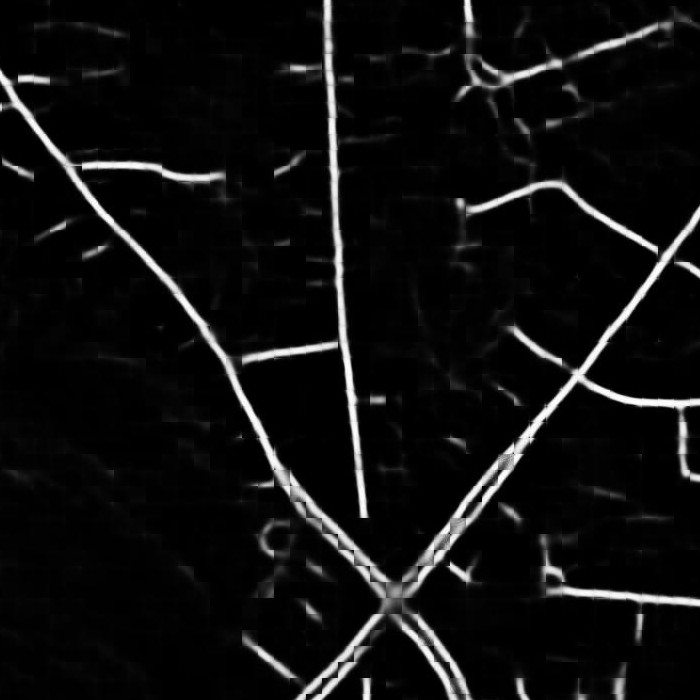
\includegraphics[width=\textwidth]{figs/appendix/pred11128870_15.jpg}
\caption{ Prediction. }
\vspace{0.2cm} % separation vertically between the subfigures
\end{subfigure}
\hspace*{\fill} % separation between the subfigures
\begin{subfigure}{0.23\textwidth}
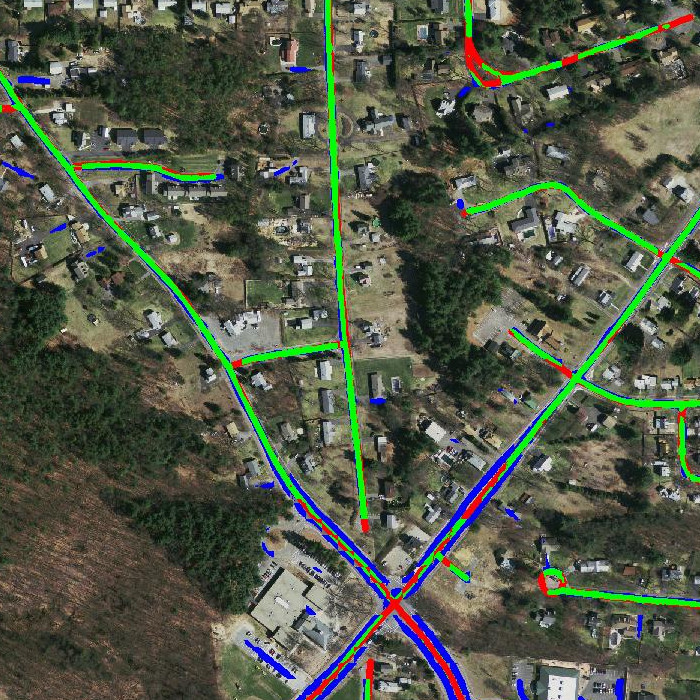
\includegraphics[width=\textwidth]{figs/appendix/hit11128870_15.jpg}
\caption{ Hits. }
\vspace{0.2cm} % separation vertically between the subfigures
\end{subfigure}
\begin{subfigure}{0.23\textwidth}
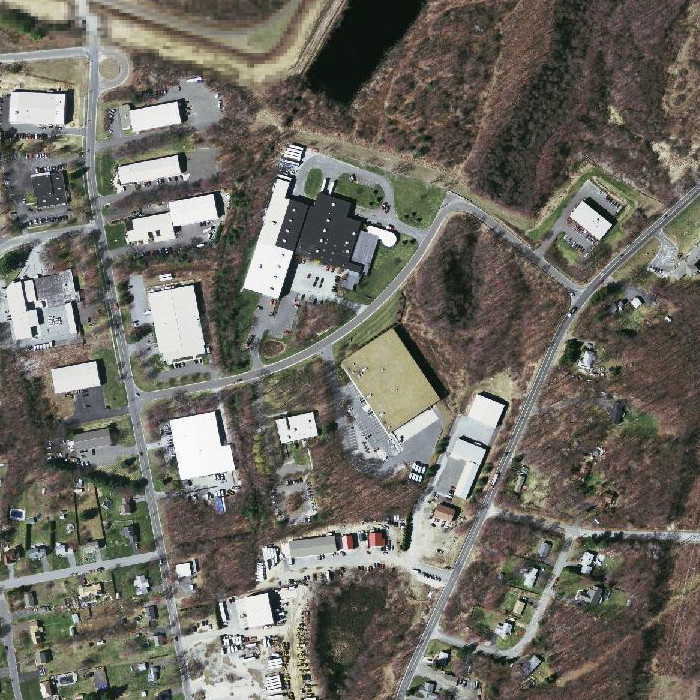
\includegraphics[width=\textwidth]{figs/appendix/img11728825_15.jpg}
\caption{ Image.}
\vspace{0.2cm} % separation vertically between the subfigures
\end{subfigure}
\hspace*{\fill} % separation between the subfigures
\begin{subfigure}{0.23\textwidth}

\includegraphics[width=\textwidth]{figs/appendix/label11728825_15.jpg}
\caption{Label}
\vspace{0.2cm} % separation vertically between the subfigures
\end{subfigure}
\hspace*{\fill} % separation between the subfigures
\begin{subfigure}{0.23\textwidth}
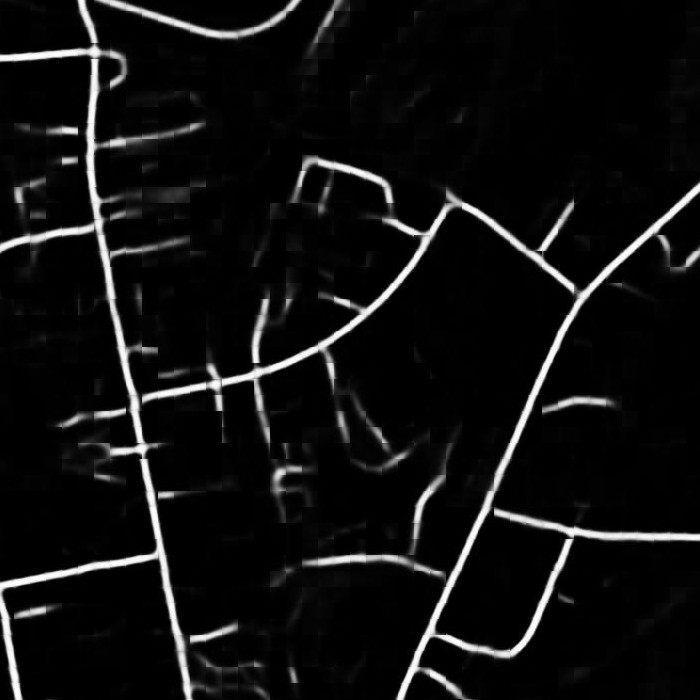
\includegraphics[width=\textwidth]{figs/appendix/pred11728825_15.jpg}
\caption{Prediction.}
\vspace{0.2cm} % separation vertically between the subfigures
\end{subfigure}
\hspace*{\fill} % separation between the subfigures
\begin{subfigure}{0.23\textwidth}
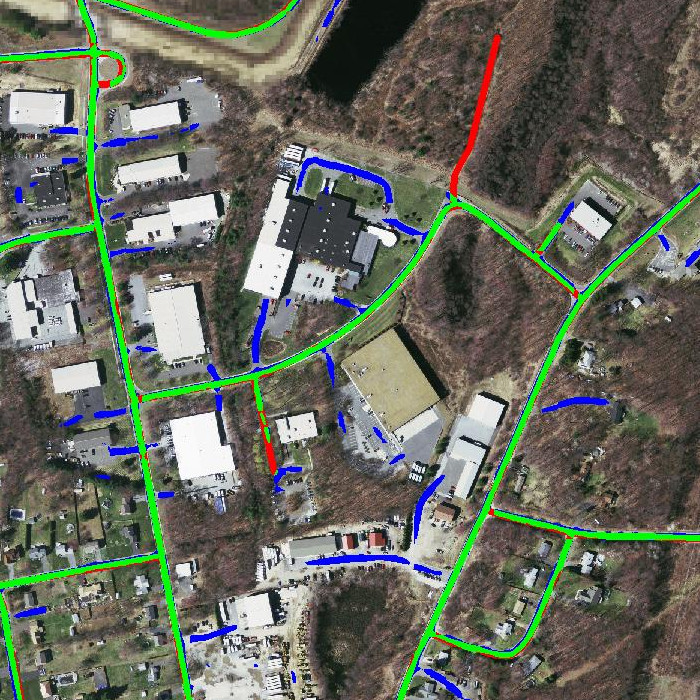
\includegraphics[width=\textwidth]{figs/appendix/hit11728825_15.jpg}
\caption{Hits.}
\vspace{0.2cm} % separation vertically between the subfigures
\end{subfigure}
\caption[Massachusetts Road extraction results 1]{Road extraction results 1 from the Massachusetts Roads Dataset.} \label{fiMass_app_results1}
\end{figure}

\begin{figure}[H]
\begin{subfigure}{0.23\textwidth}
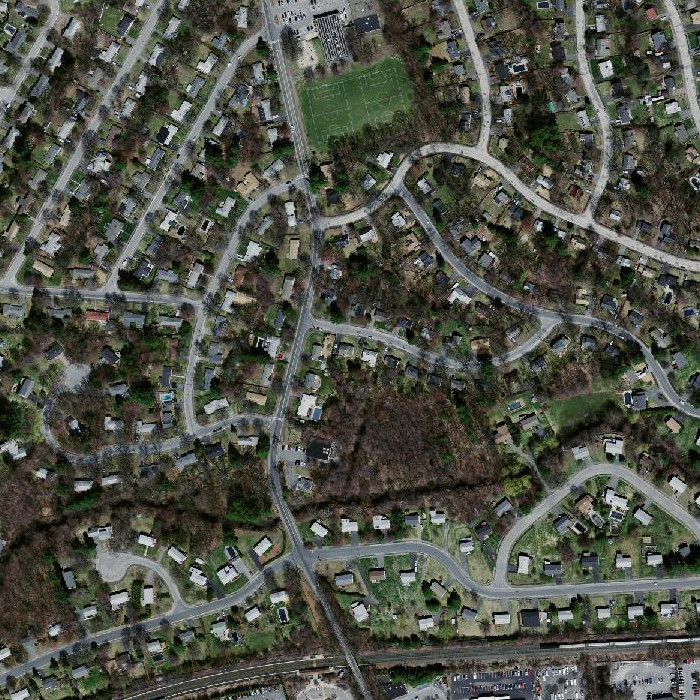
\includegraphics[width=\textwidth]{figs/appendix/img20878930_15.jpg}
\caption{ Image. }
\vspace{0.2cm} % separation vertically between the subfigures
\end{subfigure}
\hspace*{\fill} % separation between the subfigures
\begin{subfigure}{0.23\textwidth}

\includegraphics[width=\textwidth]{figs/appendix/label20878930_15.jpg}
\caption{ Label. }
\vspace{0.2cm} % separation vertically between the subfigures
\end{subfigure}
\hspace*{\fill} % separation between the subfigures
\begin{subfigure}{0.23\textwidth}
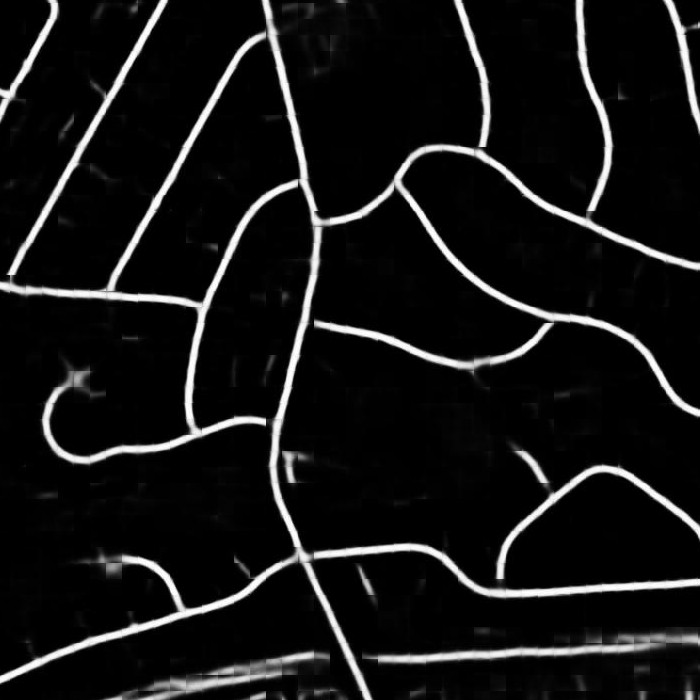
\includegraphics[width=\textwidth]{figs/appendix/pred20878930_15.jpg}
\caption{ Prediction. }
\vspace{0.2cm} % separation vertically between the subfigures
\end{subfigure}
\hspace*{\fill} % separation between the subfigures
\begin{subfigure}{0.23\textwidth}
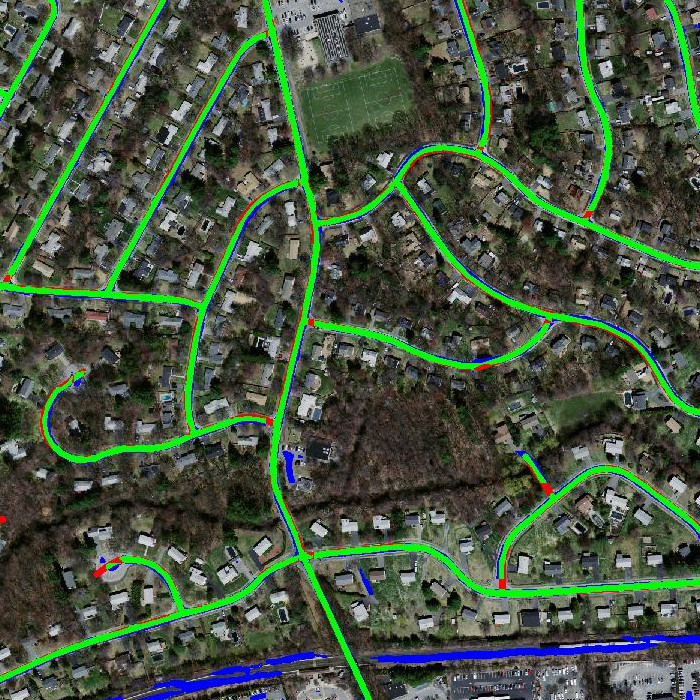
\includegraphics[width=\textwidth]{figs/appendix/hit20878930_15.jpg}
\caption{ Hits. }
\vspace{0.2cm} % separation vertically between the subfigures
\end{subfigure}
\begin{subfigure}{0.23\textwidth}
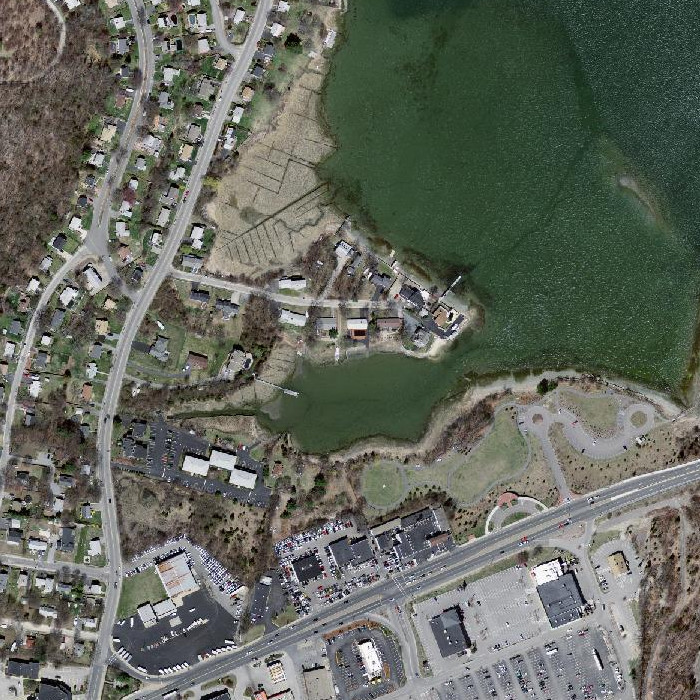
\includegraphics[width=\textwidth]{figs/appendix/img24628885_15.jpg}
\caption{ Image.}
\vspace{0.2cm} % separation vertically between the subfigures
\end{subfigure}
\hspace*{\fill} % separation between the subfigures
\begin{subfigure}{0.23\textwidth}
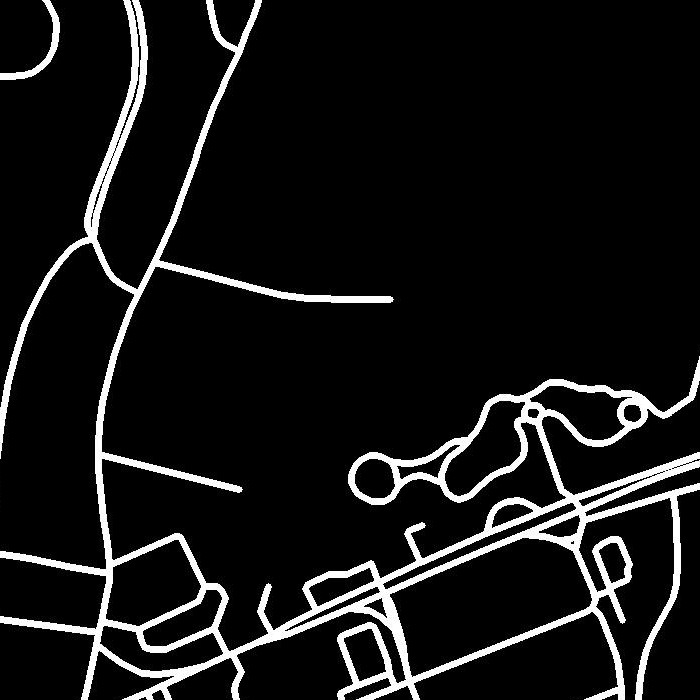
\includegraphics[width=\textwidth]{figs/appendix/label24628885_15.jpg}
\caption{Label}
\vspace{0.2cm} % separation vertically between the subfigures
\end{subfigure}
\hspace*{\fill} % separation between the subfigures
\begin{subfigure}{0.23\textwidth}
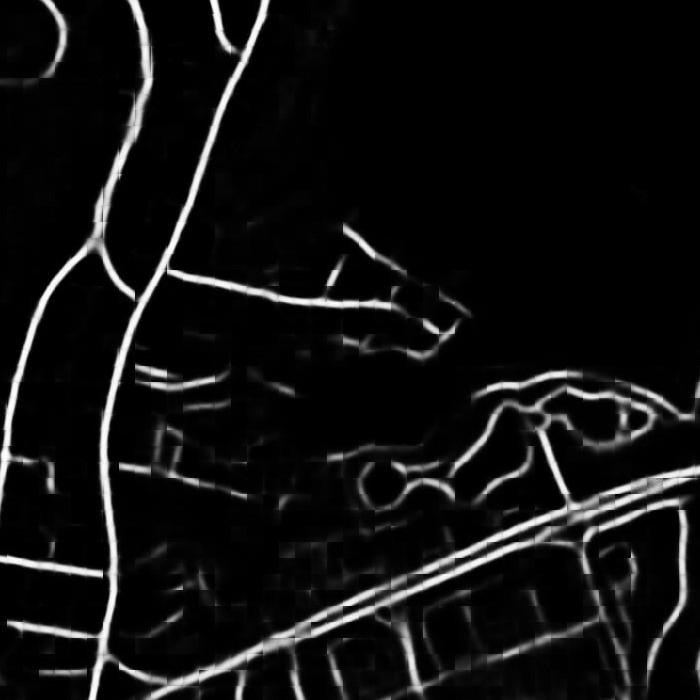
\includegraphics[width=\textwidth]{figs/appendix/pred24628885_15.jpg}
\caption{Prediction.}
\vspace{0.2cm} % separation vertically between the subfigures
\end{subfigure}
\hspace*{\fill} % separation between the subfigures
\begin{subfigure}{0.23\textwidth}
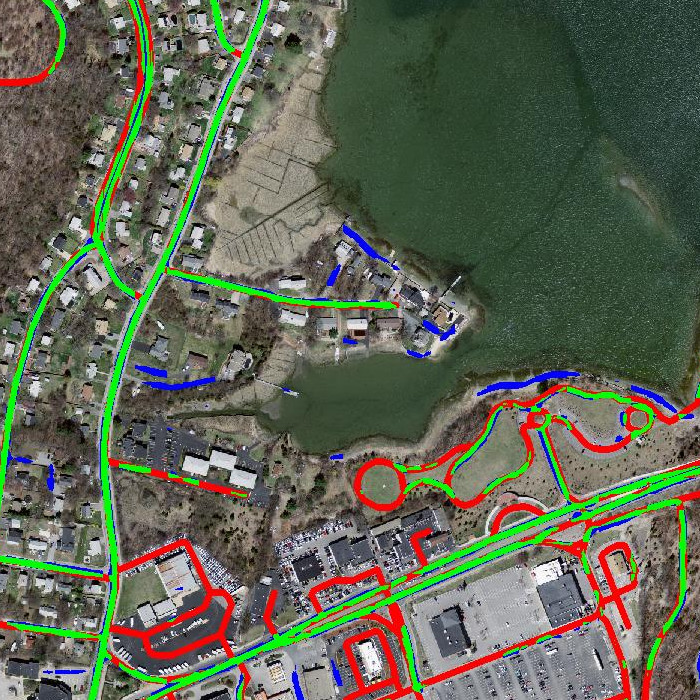
\includegraphics[width=\textwidth]{figs/appendix/hit24628885_15.jpg}
\caption{Hits.}
\vspace{0.2cm} % separation vertically between the subfigures
\end{subfigure}
\caption[Massachusetts Road extraction results 1]{Road extraction results 2 from the Massachusetts Roads Dataset.} \label{fiMass_app_results2}
\end{figure}

\section{Experiment E2 Results}
\label{app:fullE5results}

The results from Experiment E2, were summarised by plotting the final test loss and precision and breakeven point for increasing levels of omission noise. In this appendix, the test loss figures for every noise rate is shown in Figure \ref{fig:E2_all_lc}, while the precision and recall curves are depicted in Figure \ref{fig:E2_all_pr}. Each plot is the average from 10 separate runs.\\

\begin{figure}[H]
\begin{subfigure}{0.31\textwidth}
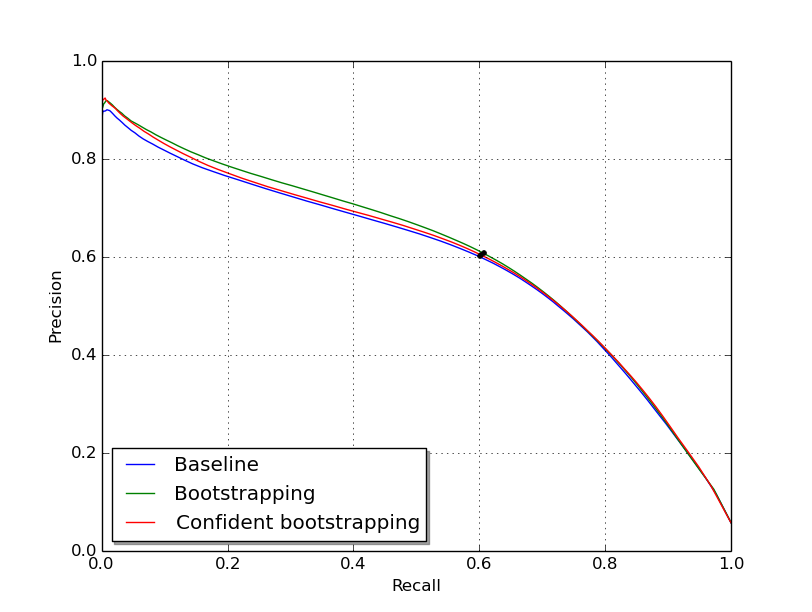
\includegraphics[width=\textwidth]{figs/E2/pr_0.png}
\caption{ 0\% } \label{fig:app_E2_0_pr}
\vspace{0.1cm} % separation vertically between the subfigures
\end{subfigure}
\hspace*{\fill} % separation between the subfigures
\begin{subfigure}{0.31\textwidth}
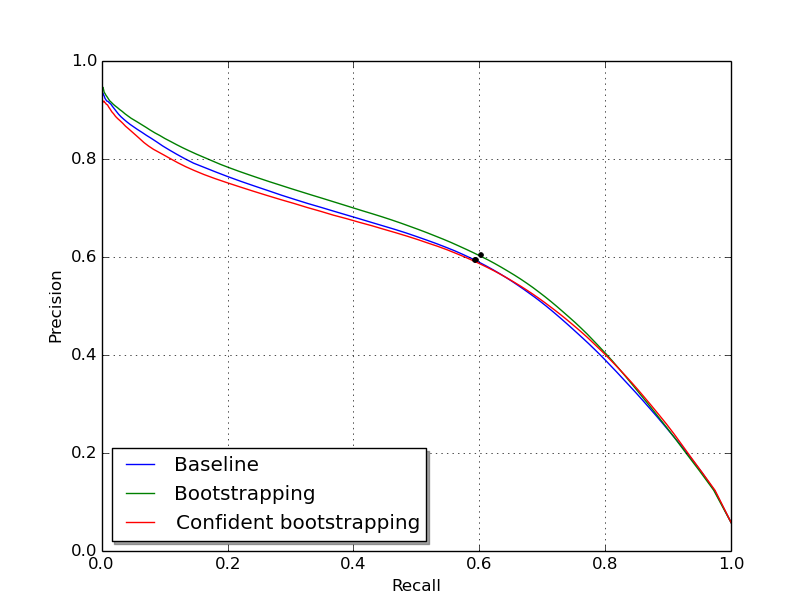
\includegraphics[width=\textwidth]{figs/E2/pr_1.png}
\caption{10\% } \label{fig:app_E2_1_pr}
\vspace{0.1cm} % separation vertically between the subfigures
\end{subfigure}
\hspace*{\fill} % separation between the subfigures
\begin{subfigure}{0.31\textwidth}
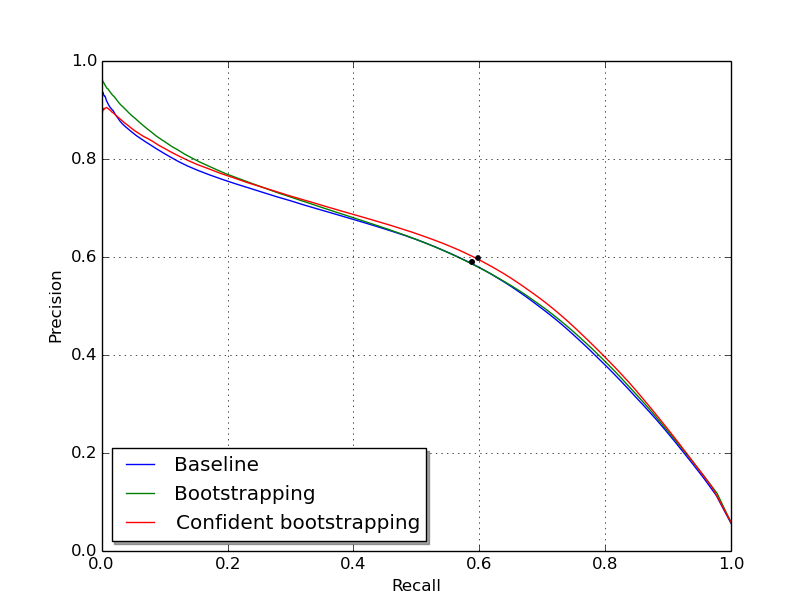
\includegraphics[width=\textwidth]{figs/E2/pr_2.png}
\caption{20\% } \label{fig:app_E2_2_pr}
\vspace{0.1cm} % separation vertically between the subfigures
\end{subfigure}
\begin{subfigure}{0.31\textwidth}
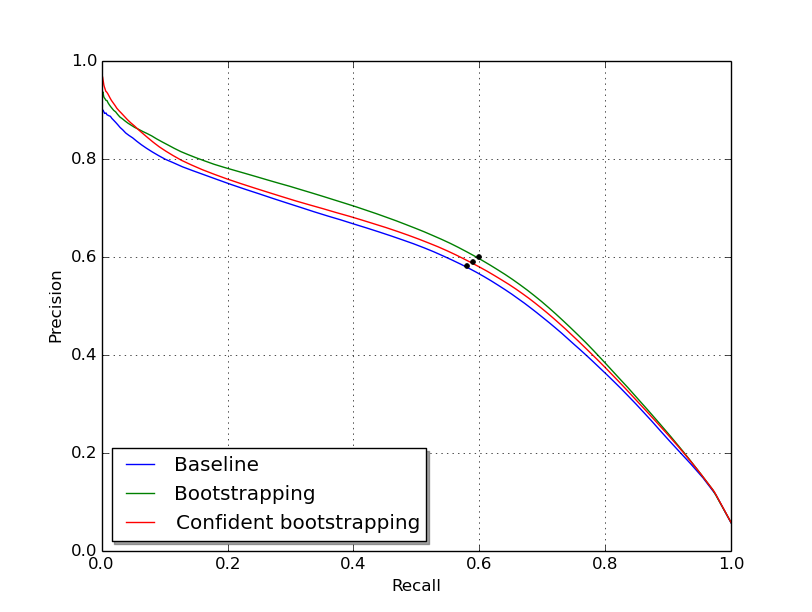
\includegraphics[width=\textwidth]{figs/E2/pr_3.png}
\caption{ 30\%} \label{fig:app_E2_3_pr}
\vspace{0.1cm} % separation vertically between the subfigures
\end{subfigure}
\hspace*{\fill} % separation between the subfigures
\begin{subfigure}{0.31\textwidth}
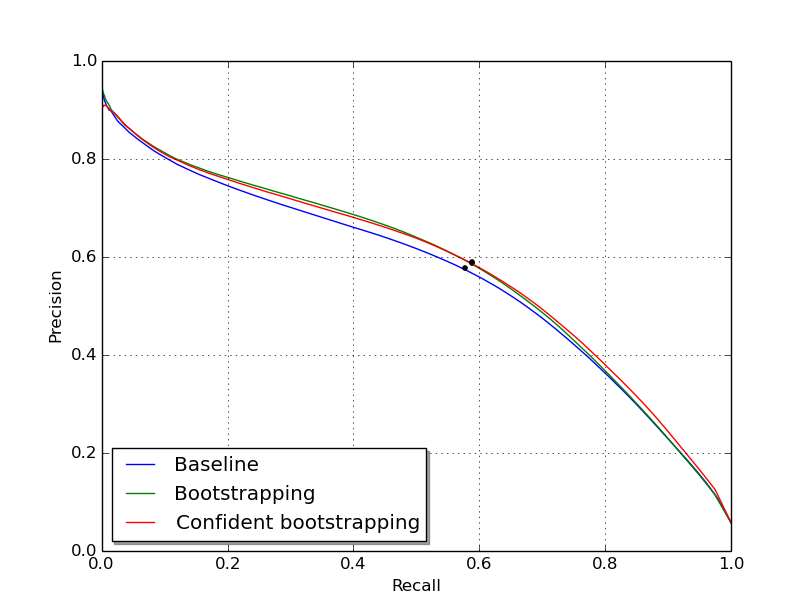
\includegraphics[width=\textwidth]{figs/E2/pr_4.png}
\caption{40\%} \label{fig:app_E2_4_pr}
\vspace{0.1cm} % separation vertically between the subfigures
\end{subfigure}
\caption{E5 - Precision and recall breakeven comparisons for several levels of omission noise.} \label{fig:E2_all_pr}
\end{figure}

\begin{figure}[H]
\begin{subfigure}{0.3\textwidth}
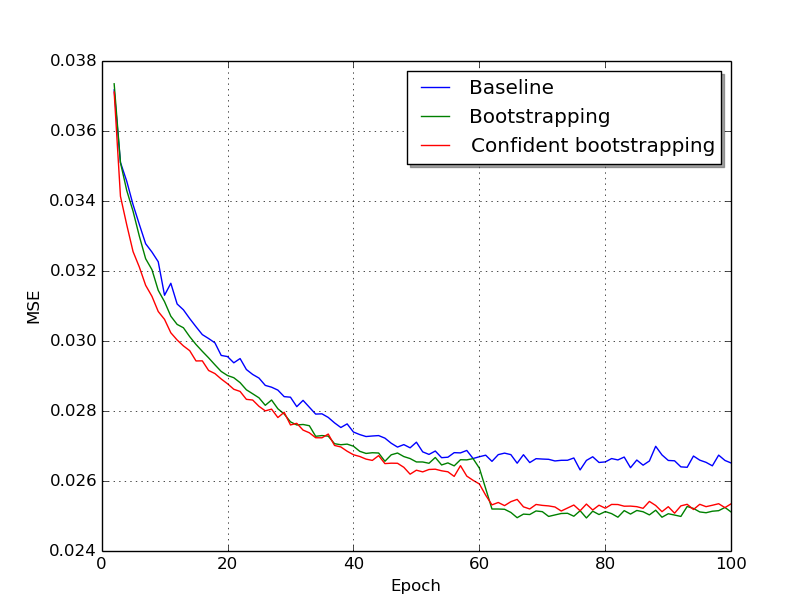
\includegraphics[width=\textwidth]{figs/E2/lc_0.png}
\caption{ 0\% } \label{fig:app_E2_0_lc}
\vspace{0.1cm} % separation vertically between the subfigures
\end{subfigure}
\hspace*{\fill} % separation between the subfigures
\begin{subfigure}{0.31\textwidth}
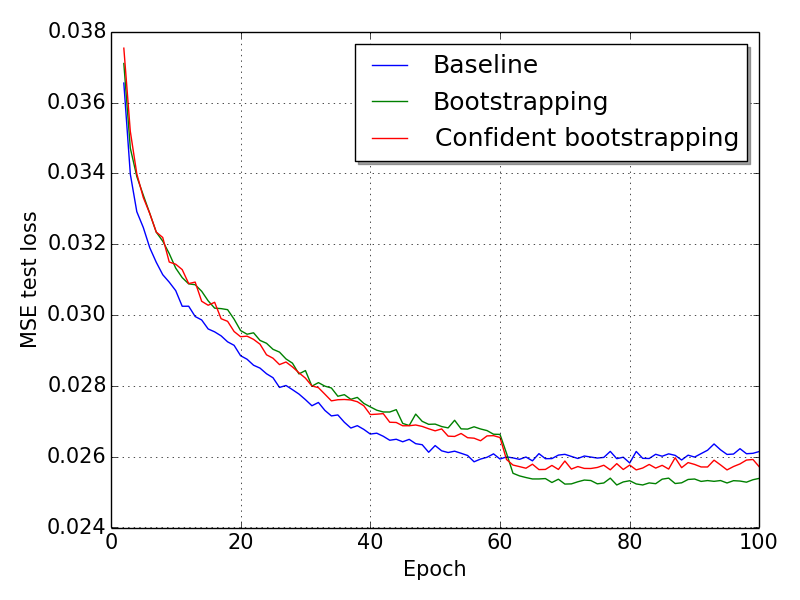
\includegraphics[width=\textwidth]{figs/E2/lc_1.png}
\caption{10\% } \label{fig:app_E2_1_lc}
\vspace{0.1cm} % separation vertically between the subfigures
\end{subfigure}
\hspace*{\fill} % separation between the subfigures
\begin{subfigure}{0.31\textwidth}
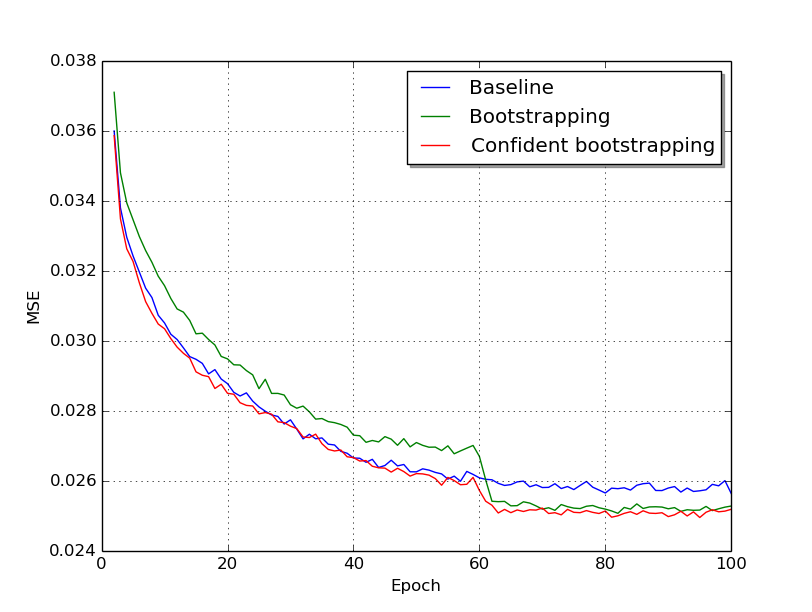
\includegraphics[width=\textwidth]{figs/E2/lc_2.png}
\caption{20\% } \label{fig:app_E2_2_lc}
\vspace{0.1cm} % separation vertically between the subfigures
\end{subfigure}
\begin{subfigure}{0.31\textwidth}
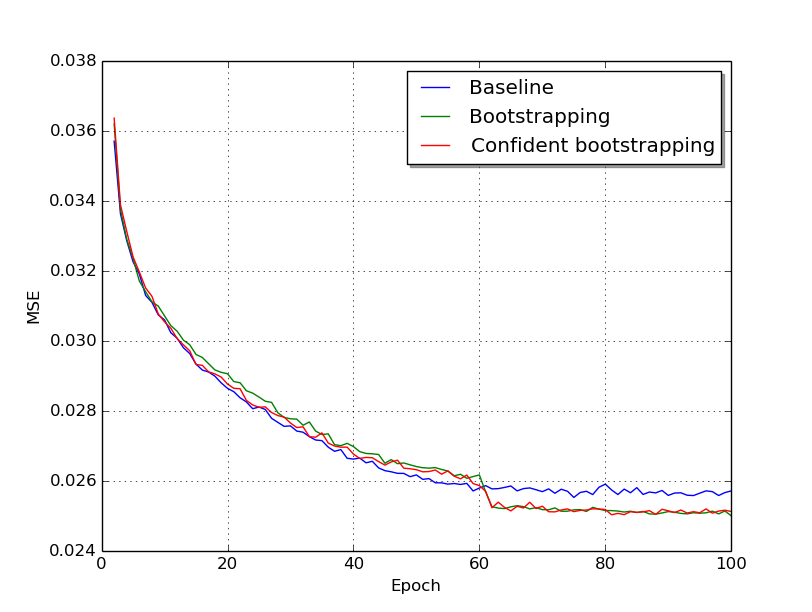
\includegraphics[width=\textwidth]{figs/E2/lc_3.png}
\caption{ 30\%} \label{fig:app_E2_3_lc}
\vspace{0.1cm} % separation vertically between the subfigures
\end{subfigure}
\hspace*{\fill} % separation between the subfigures
\begin{subfigure}{0.31\textwidth}
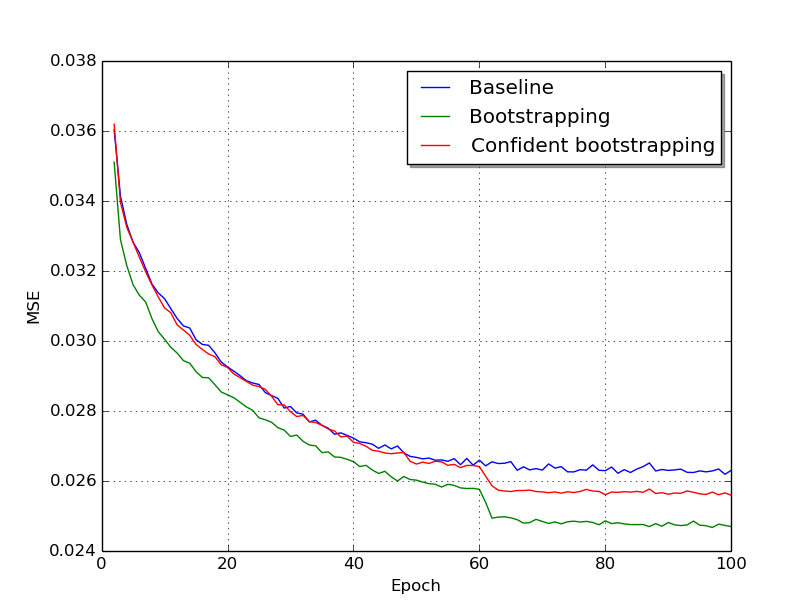
\includegraphics[width=\textwidth]{figs/E2/lc_4.png}
\caption{40\%} \label{fig:app_E2_4_lc}
\vspace{0.1cm} % separation vertically between the subfigures
\end{subfigure}
\caption{E2 - Test loss comparisons for several levels of omission noise.} \label{fig:E2_all_lc}
\end{figure}


\section{TODOs which apply to entire thesis}
\todo[inline]{Remove this part!}
\begin{itemize}
\item Rest of results.
\item Student t test for results. To see if results are significant, or convincing is the better word.uncertainty for every pair.
\item Update figures
\item proof read
\item Confirm that number of stored weights correspond to weight calculation in google drive 
\item Explain the accuracy improvemnets in results discussion?
\item Road extraction, road detection, semantic segmentation, patch-based. Need clarity, and really good understanding of these terms. Check for misuse of these terms!
\item Read sukhbaatar updated paper
\item Acronym CNN, is ok. But only defined once? Or once per chapter.
\item Check that installation guides and dependencies are correct - Appendix A, B, C
\item Proof read for incorrect future tense
\item Where by is more appropriate than for
\item Check if repetitions of mnih and saito is unclear
\end{itemize}
